%File: RBM.tex
%Date: Mon Dec 30 21:12:54 2013 +0800
%Author: Yuxin Wu <ppwwyyxxc@gmail.com>


\subsection{CRBM}

\begin{frame}{CRBM}
  \begin{itemize}
    \item \textbf{Restricted Boltzmann Machine} is a generative stochastic two-layer neural network.

    \item \textbf{Continuous RBM} extends RBM to real-valued inputs.
      \pause
    \item RBM has a ability to reconstruct a layer similar to input layer.
      The difference between the two layers can be a used to measure the fitness of an input to the model.

    \item Therefore, RBM can be a substituion to GMM.
  \end{itemize}


  \begin{reference}{4mm}{85mm}
Chen, Hsin and Murray, Alan F, 2003,
Continuous restricted Boltzmann machine with an implementable training algorithm
  \end{reference}
\end{frame}

\begin{frame}{Results}
  Results of CRBM, tested with 5 secs
  of utterance.
  \begin{center}
    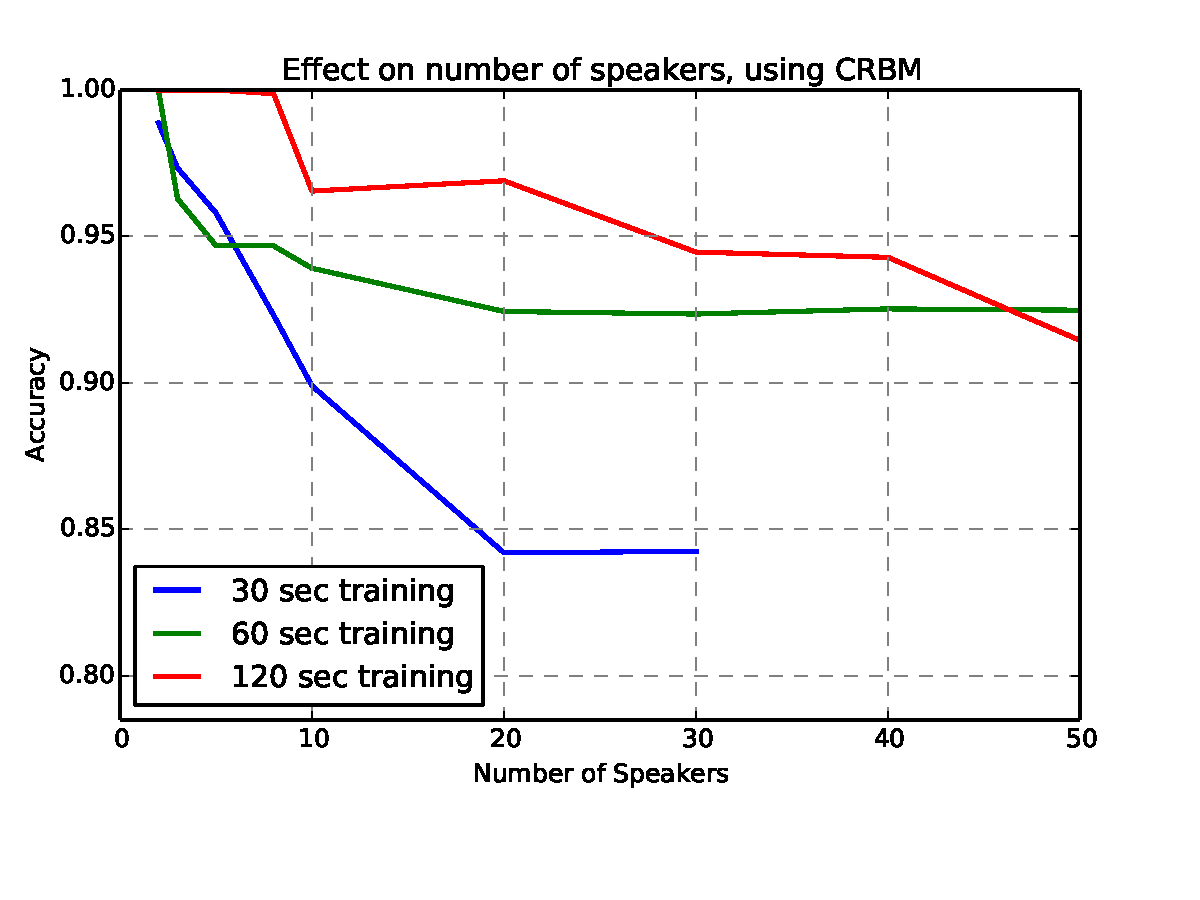
\includegraphics[width=0.7\textwidth]{res/crbm.pdf}
  \end{center}
\end{frame}

